% !TEX encoding = UTF-8 Unicode
% !TEX root = rapport.tex

\chapter{Initiatives et solutions}\label{initiatives_actuelles}

\section{Initiatives des pouvoirs publics}

\subsection{Mesures des pouvoirs publics français}
\subsubsection{Le C2i}

Mis en place à partir de la rentrée universitaire 2003
\cite{circulaire_c2i}, le certificat informatique et internet (C2i)
vise à encadrer la formation des étudiants aux technologies
informatisées et à internet par l'établissement d'un socle commun.

\begin{figure}[H]
  \centering
  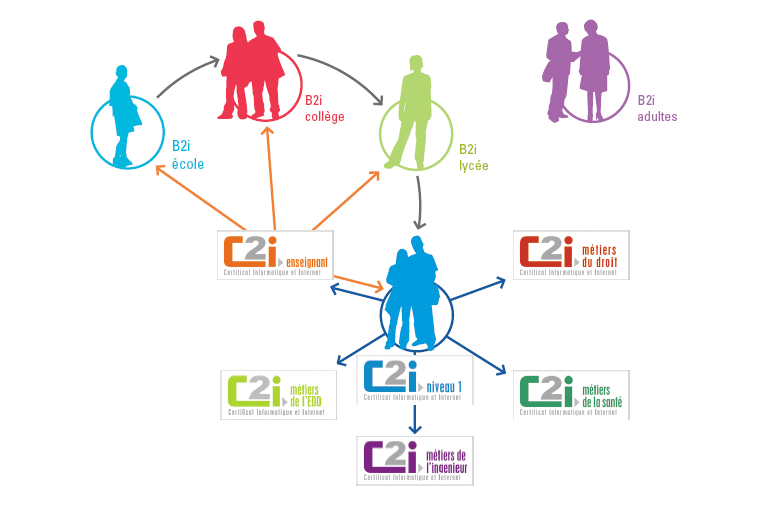
\includegraphics[width=\textwidth]{../resources/illustrations/c2i}
  \caption{Différents niveaux et spécialités du C2i}
\end{figure}

\cite{b2i_c2i}
\cite{b2i}
\cite{isn}

\subsubsection{Les opérations "ordinateurs portables"}

Les opérations \og{}ordinateurs portables\fg{} sont à la mode au
lycée. OrdiLib' en Midi-Pyrénées, Ordipass en Pays de la Loire, LoRdi
en Languedoc-Roussilon, ces initiatives des régions visent à fournir à
chaque lycéen l'accès à un ordinateur portable personnel.

\cite{portables35}
\cite{portables60}
\cite{portables40}


\subsubsection{Le rapport \og{}Refondons l'école de la république\fg{}}

Nous avons vu différentes actions mené par le gouvernement ou les
régions afin d'une part de former les étudiants au NTIC et d'autres
part de favoriser l'utilisation des NTIC dans le système éducatif. Nous
allons maintenant nous intéresser aux propositions pour l'avenir de
l'éducation à travers la concertation \og{}Refondons l'école de la
république\fg{} confié par le gouvernement Ayrault à Nathalie Mons, Christian
Forestier, François Bonneau et Marie-Françoise Colombani. Il ressort à
travers se rapport plusieurs thèmes tels que \og{}apprendre à
apprendre\fg{}, \og{}une appropriation active des langues\fg{},
\og{}usages pédagogiques du numérique en primaire\fg{}, \og{}une
évaluation positive, plutôt qu'une note sanction\fg{}… Ces différents
thèmes sont des points d'interrogation cruciaux pour l'école de demain,
nous regretterons cependant un manque de mesures concrètes. Nous
pouvons tout de même relevé la volonté d'inscrire dans la loi \og
l'éducation au médias et à l'information\fg{}, de mettre en place un plan
pour l'éducation numérique au primaire, de former les enseignants aux
usages pédagogiques du numérique, de mettre en place une politique
publique de recherche dans le cadre des applications pédagogiques du
numérique.


\subsection{Mesures des pouvoirs publics internationaux}
Forum mondial sur l’éducation \cite{educ_forum}
Les TIC au service de l’éducation \cite{tics}
Un regard sur la trajectoire de l’informatique éducative au Brésil \cite{peixoto2006regard}
Willem J. PELGRUM, Arian T. SCHIPPER, "Indicators of computer integration in education" \cite{pelgrum1993indicators}


\section{Initiatives d'autres acteurs}

D'autres actions, souvent plus radicales ont lieu à travers le monde. Elles sont pour la plupart menées au sein de laboratoires d'informatique. Ces projets amènent à une réelle remise en question du système éducatif et plus généralement à des réflexions poussées sur les méthodes d'apprentissage.

\subsection{Actions concrètes}

\subsubsection{One Laptop Per Child}

Nicholas Negroponte est à l'origine du projet OLPC\footnote{OLPC : One Laptop Per Child}. Il est Professeur au MIT depuis 1966 après avoir obtenu un diplôme d'architecture dans ce même établissement. Il fonde et devient président du MIT MediaLab en 1985 et lance un magazine spécialisé dans l'informatique (Wired Magazine) en 1993.

Lors de son départ du poste de président du MIT Medialab dans les années 2000, Nicholas Negroponte fait le choix de s'investir dans un projet d'envergure lui permettant d'exploiter son réseau de contacts établi avec son poste précédent. C'est en 2005 qu'est né le projet OLPC.

\begin{figure}[H]
  \centering
  
\includegraphics[width=.5\textwidth]{../resources/illustrations/OLPC_logo}
  \caption{Logo projet OLPC}
\end{figure}

OLPC est un projet éducatif visant à s'occuper de l'éducation en agissant sur les enfants plutôt que sur la structure éducative. Le projet est composé de plusieurs points : 



\begin{itemize}
  \item la conception et la production d'un ordinateur,
  \item la distribution aux enfants,
  \item la mise à disposition d'une connexion internet haut débit.
\end{itemize}

OLPC s'appuie sur une structure associatif, à but non lucratif, dans le but d'assurer la bonne lisibilité de son but moral initial. Nicholas Negroponte annonce lors d'un discours \cite{ted_olpc_2008} que le fait d'avoir un but moral clair lui à permis d'impliquer à son projet de nombreuses personnalités qui n'auraient pas accepté si la structure n'était pas à but non lucrative.

Nicholas Negroponte ayant déjà travaillé avec Seymour Papert, ce projet est clairement basé sur la philosophie du constructionnisme\footnote{Voir section \ref{sec:solutions} page \pageref{sec:solutions}}.

Le XO est l'ordinateur développé par l'équipe du projet. Les principaux points du cahier des charges étaient les suivants : 

\begin{description}
  \item [Le prix], idéalement inférieur à 100\$. Il pourra être atteint en maximisant le volume de fabrication. L'ordinateur est ensuite vendu à prix coutant aux pays souhaitant équiper leurs élèves.
  \item [Lecture en plein soleil], permise grâce à un écran hybride fournissant deux modes de fonctionnement : mode e-paper (n\& b) lisible au soleil, et mode normal LCD. La vente d'ordinateur étant effectuée principalement dans des pays en voie de développement, cette fonctionnalité permet de faciliter l'utilisation extérieur et d'accroitre la longévité de la batterie là où les sources d'électricité peuvent être rares.
  \item [Autonomie de la batterie], assuré par l'intégration de composants peu gourmands en énergie et, comme indiqué ci-avant, par l'écran e-paper.
  \item [Réseau maillé], il permet de ne pas centraliser l'accès au réseau. Il est donc possible à des écoliers de pays émergents de rester connecté à l'école et à la maison sans construire de grosses infrastructures : le réseau est repartagé par chaque pair connectée.
\end{description}

\begin{figure}[H]
  \centering
  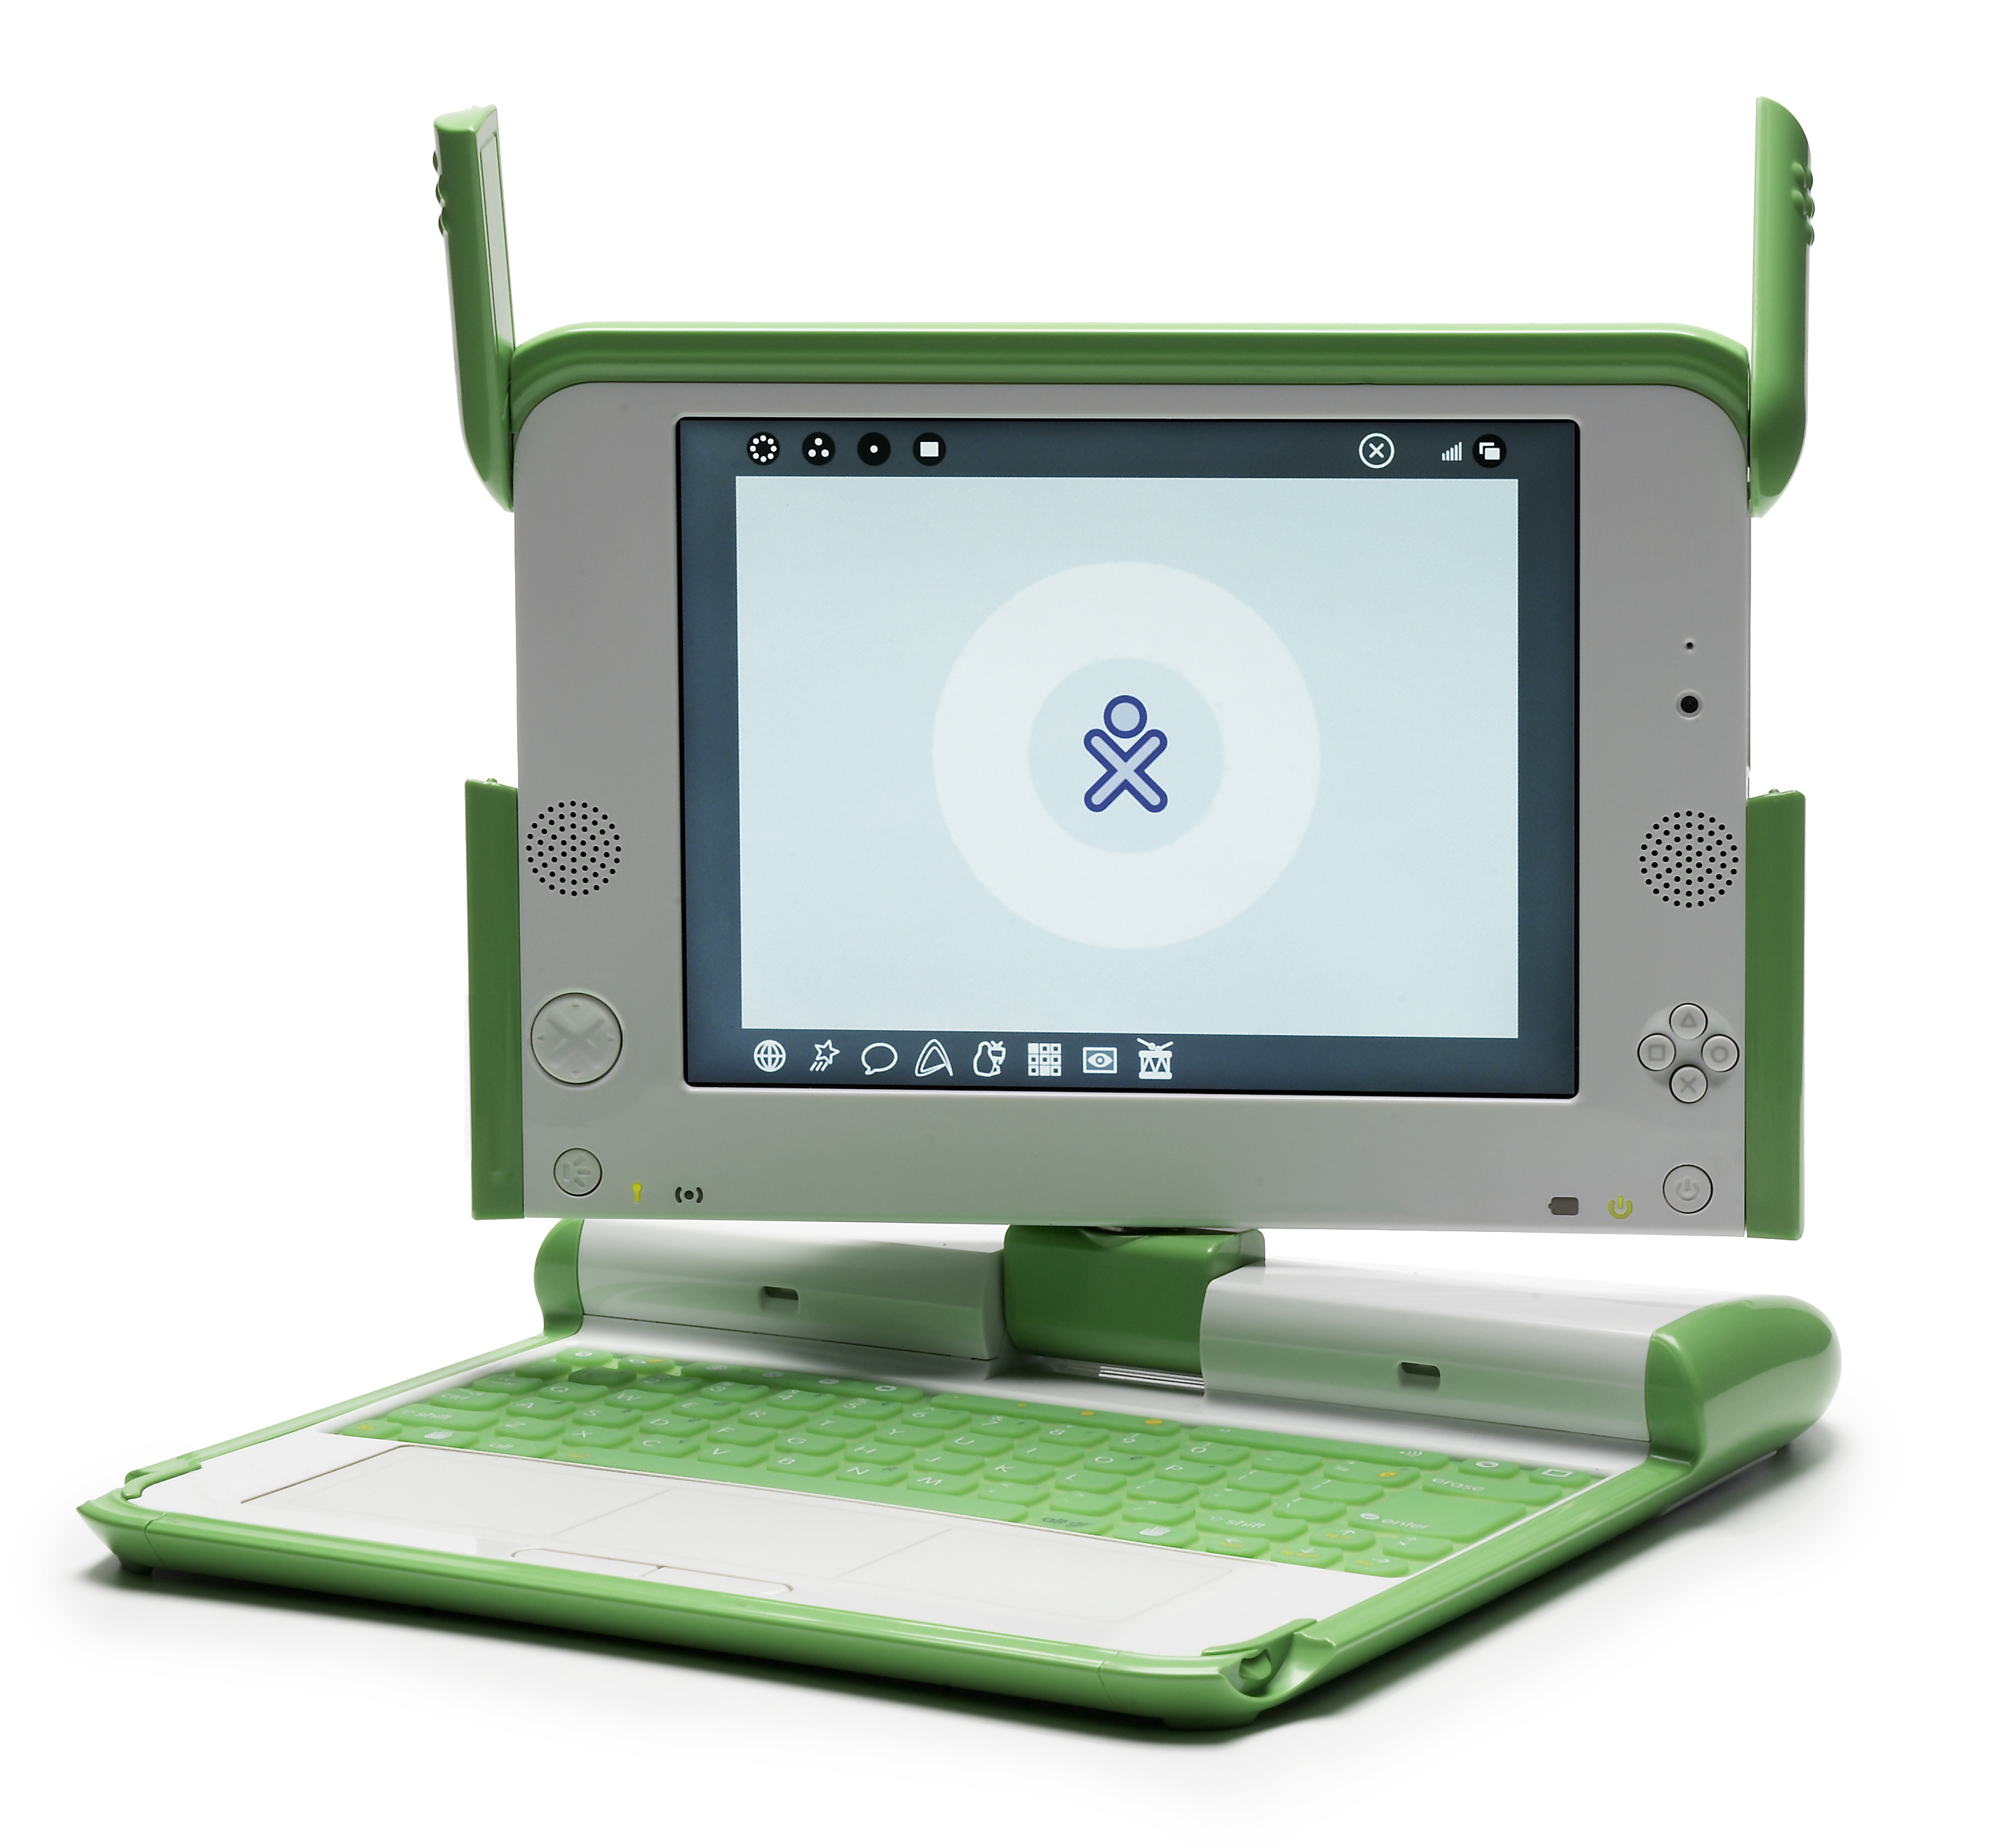
\includegraphics[width=.6\textwidth]{../resources/illustrations/olpc2}
  \caption{XO : ordinateur OLPC}
\end{figure}
\begin{minipage}{.5\linewidth}
  \begin{figure}[H]
    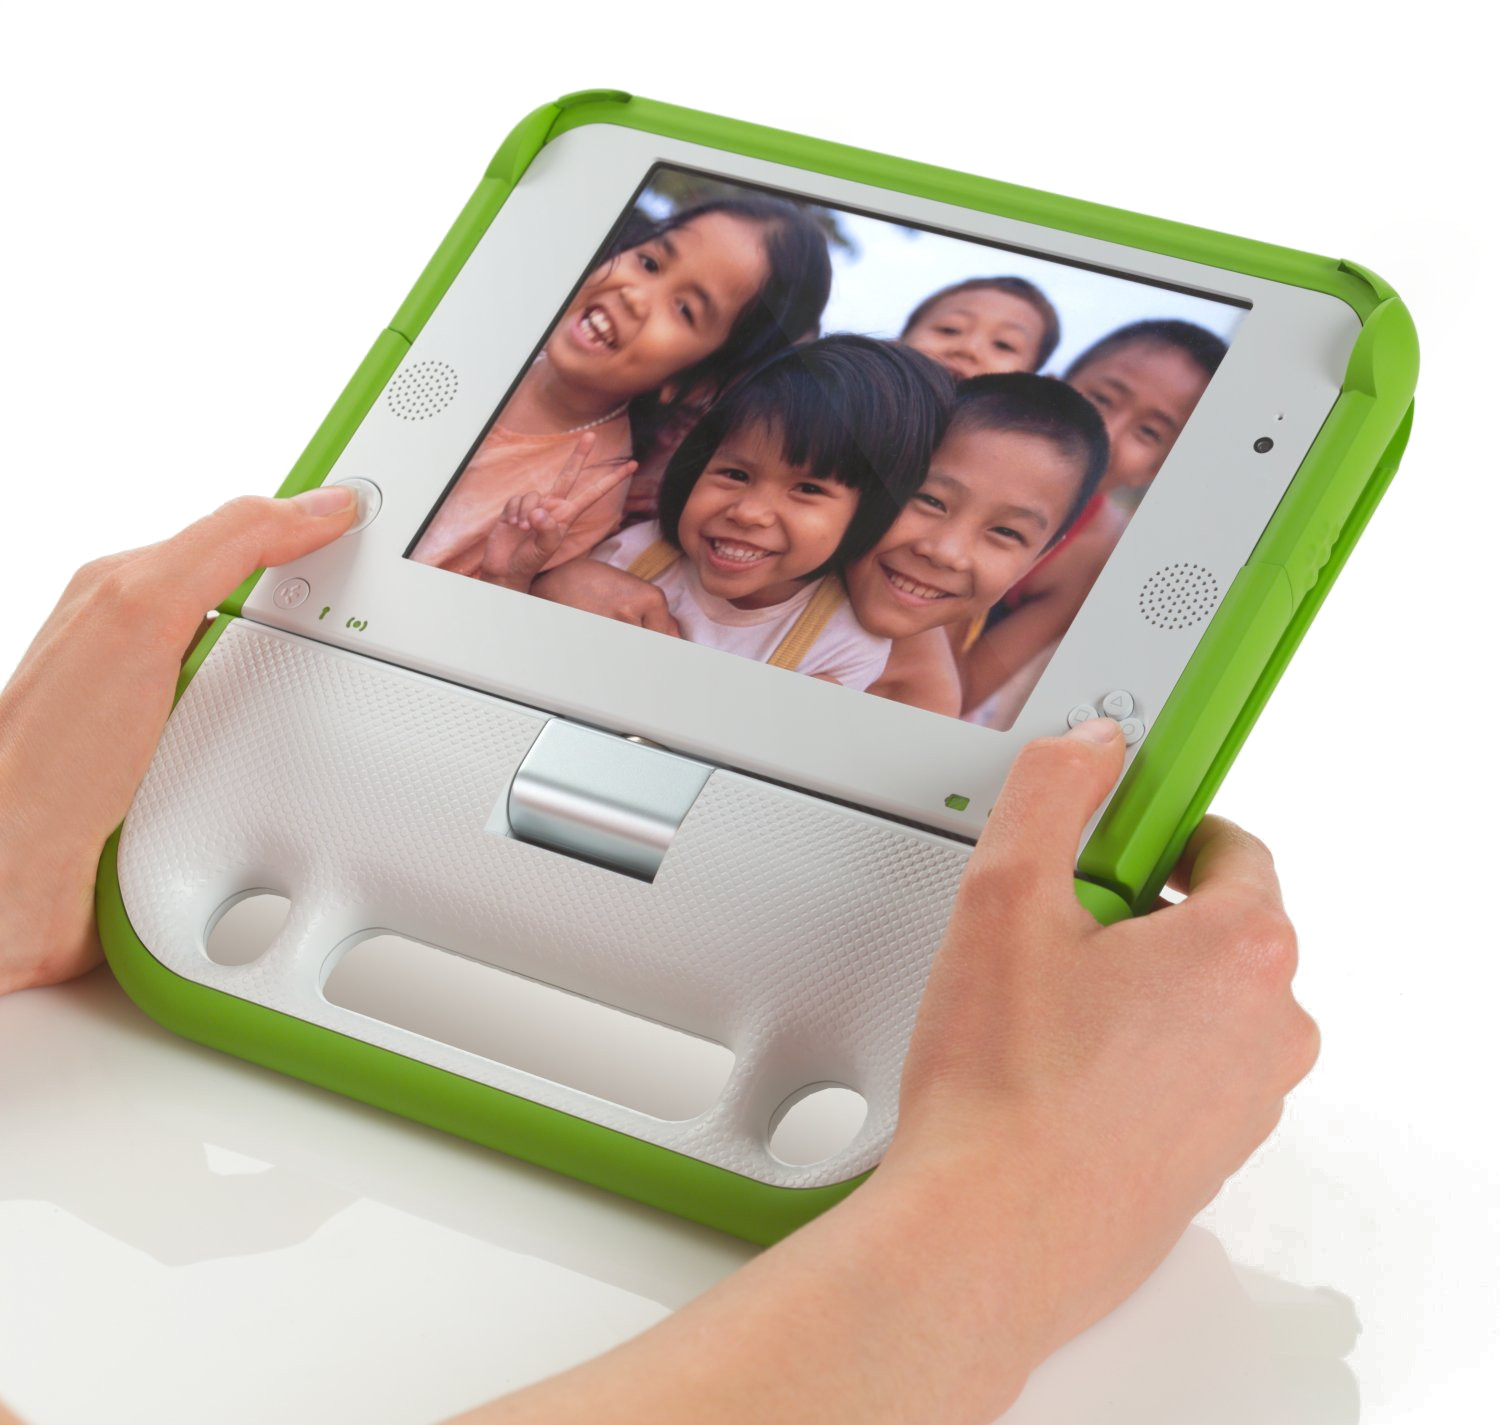
\includegraphics[width=\textwidth]{../resources/illustrations/olpc1}
    \caption{XO : mode Tablet}
  \end{figure}
\end{minipage}
\begin{minipage}{.5\linewidth}
  \begin{figure}[H]
    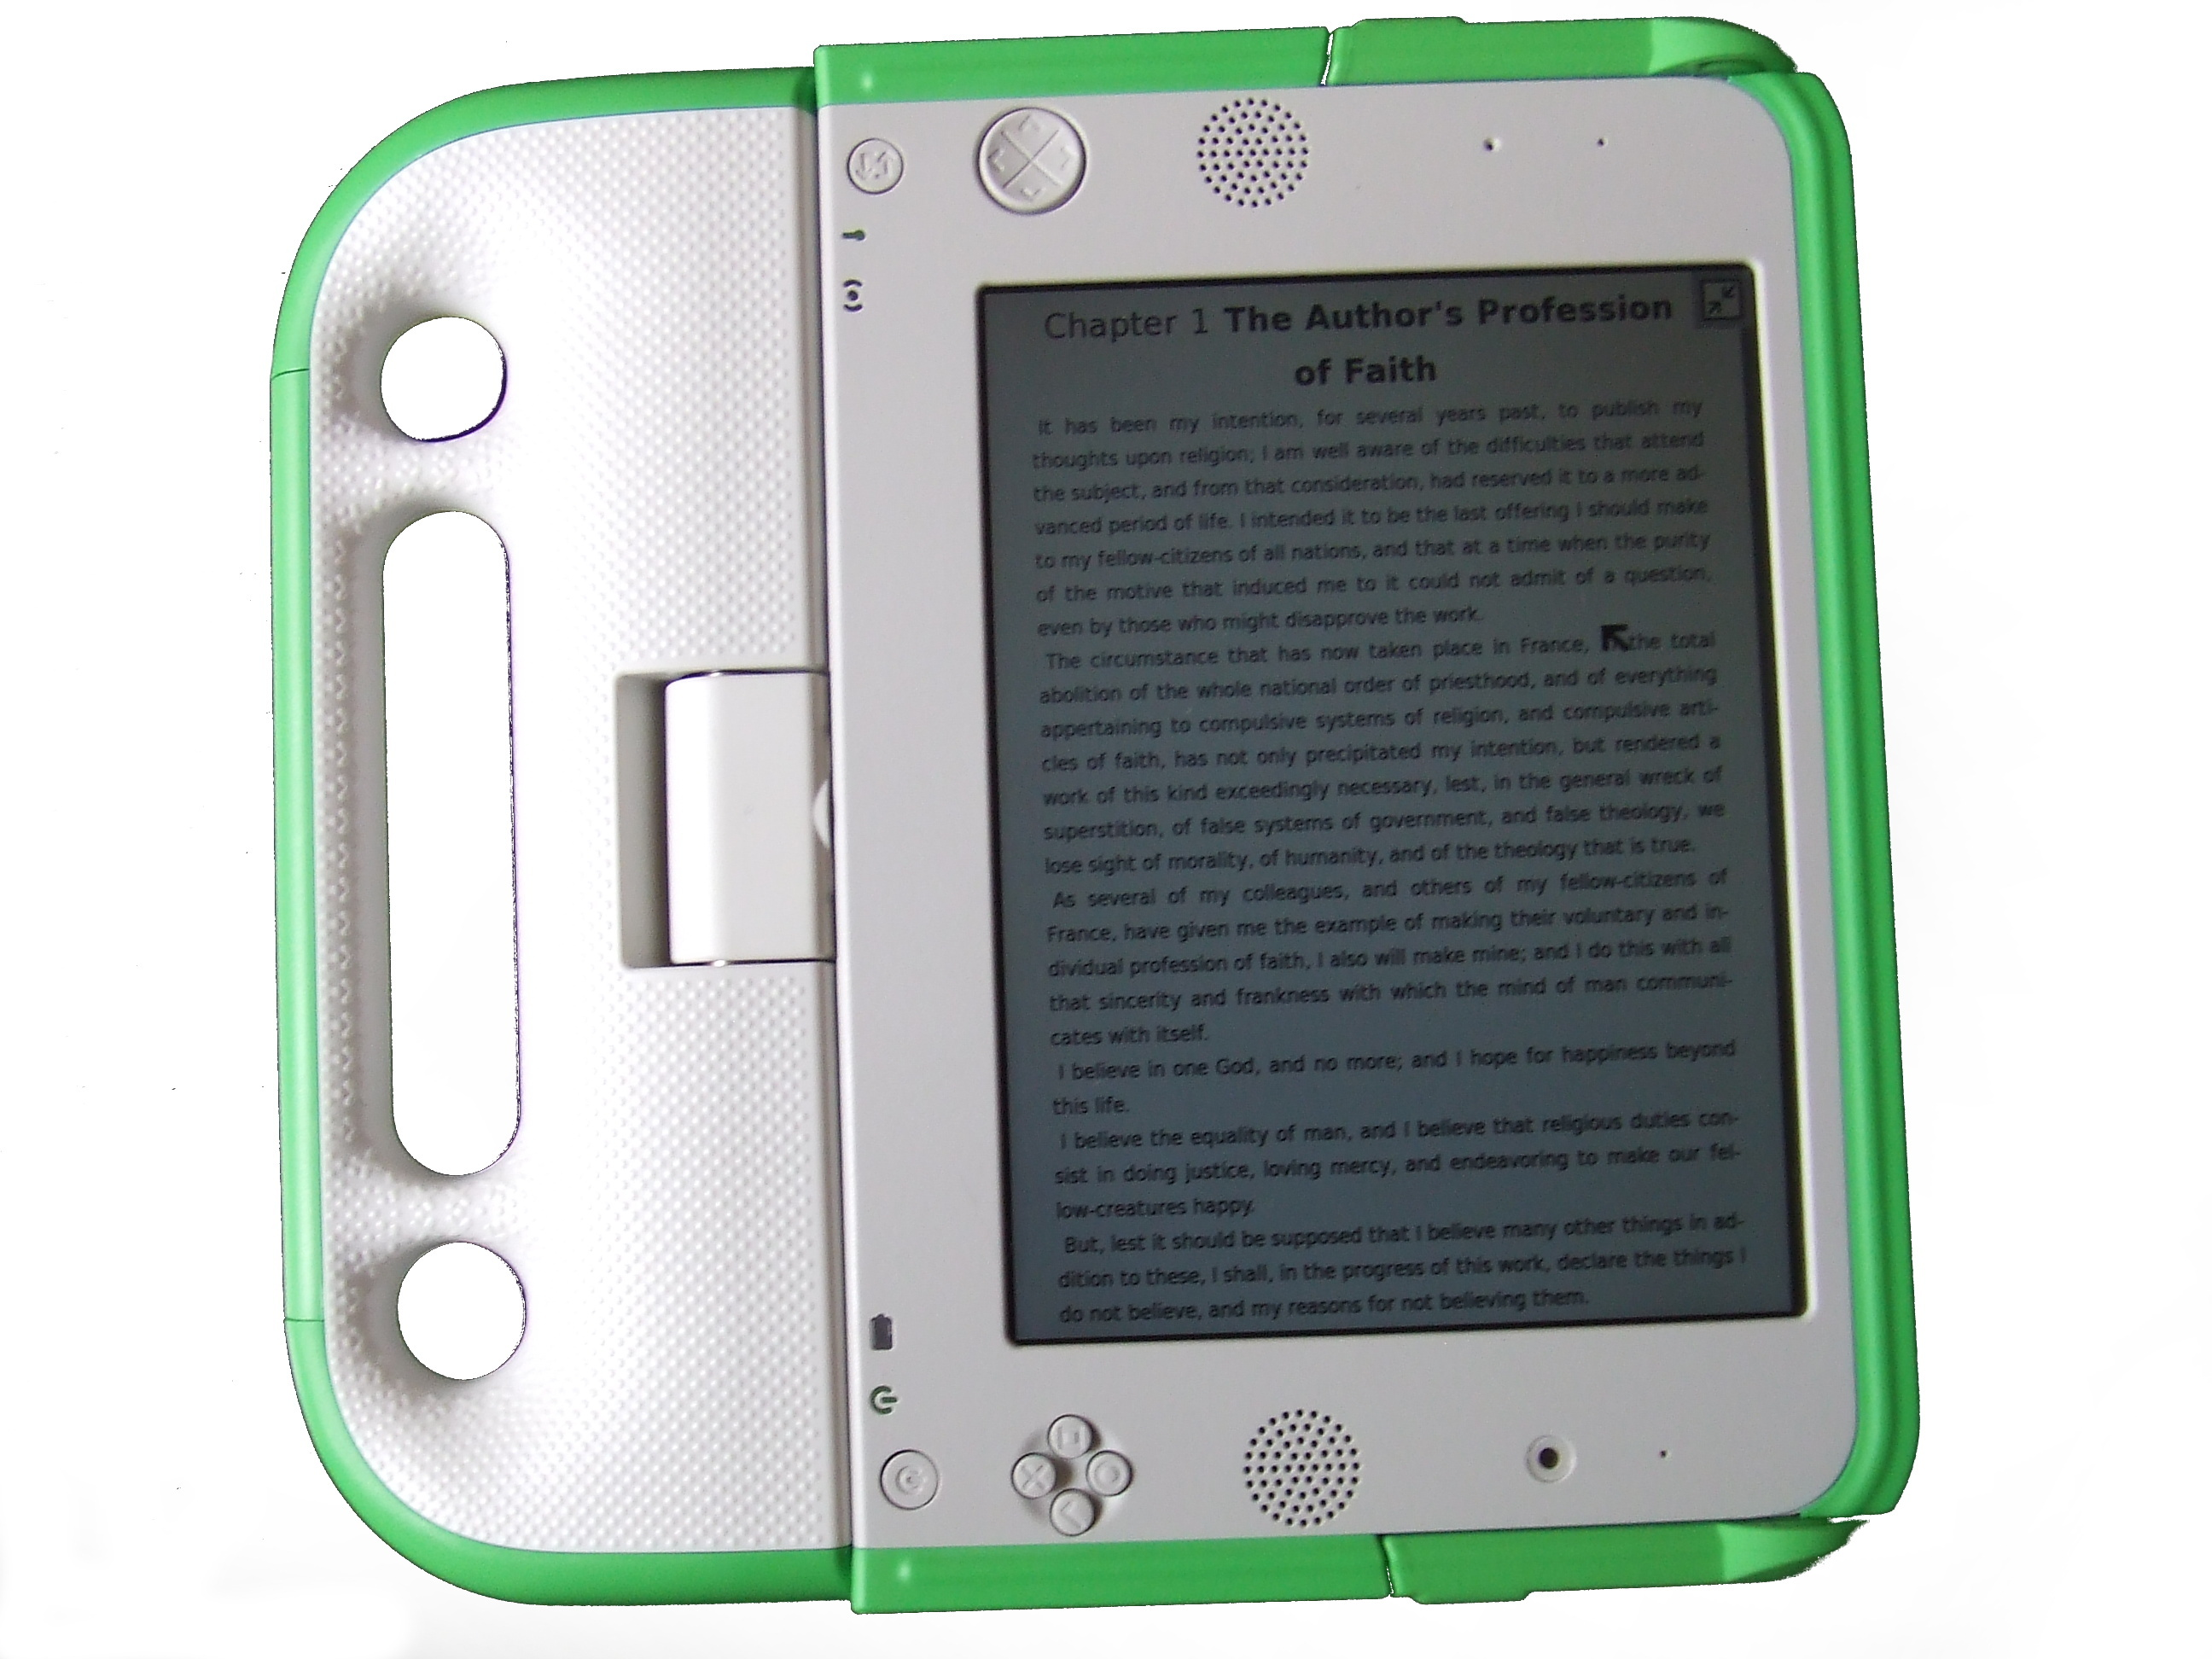
\includegraphics[width=\linewidth]{../resources/illustrations/olpc_display}
    \caption{XO : écran e-paper}
  \end{figure}
\end{minipage}



\subsubsection{e-learning / e-teaching}
\textit{Moodle -- AI-class}
Les plate-formes d'apprentissage en ligne \og{}e-learning\fg{} tels
que Moodle, udacity, kanacademy, coursera, MIT Open Courseware, etc.,
émergent depuis ces dernières années. Ce type d'apprentissage offre l'avantage d'être peu
coûteux, flexible dans la gestion du temps d'apprentissage, largement
accessible. Loin de remplacer l'enseignement traditionnel, ce type
d'apprentissage offre un complément voir un support à celui-ci. Ce
type de support est souvent utilisé pour de la formation continue
qu'elle soit professionnel ou personnelle.

\subsubsection{Auto-apprentissage}
\textit{Hole in the wall}

\section{Solutions}
\label{sec:solutions}

Interactions entre professeur et élèves
Révision des programmes
Utilisation des nouvelles technologies au service des interactions
Changements des règles de constitution des classes : pourquoi par tranches d'âge ?
Personnalisation des parcours en fonction des envies des élèves.

\subsection{Classification des élèves par besoins / capacités  et non par tranche d'âge}
\subsection{Amélioration de la pertinence des évaluations}
\subsection{Prise en compte des besoins de coopération sans parler de triche}

